% Source: Code/ML_overlay/ir_rgb_registration/paper/ml_overlay_report_materials/ir_rgb_registration_report/figures/fig_coarse_to_fine.tex
\documentclass[tikz,border=10pt]{standalone}
\usepackage{tikz}
\usetikzlibrary{arrows.meta,positioning,calc,shapes.geometric}

\definecolor{garnet}{RGB}{115,0,10}
\definecolor{rose}{RGB}{204,46,64}
\definecolor{atlantic}{RGB}{70,106,159}
\definecolor{congaree}{RGB}{31,65,77}
\definecolor{horseshoe}{RGB}{101,120,11}
\definecolor{black90}{RGB}{54,54,54}
\definecolor{black50}{RGB}{162,162,162}

\begin{document}
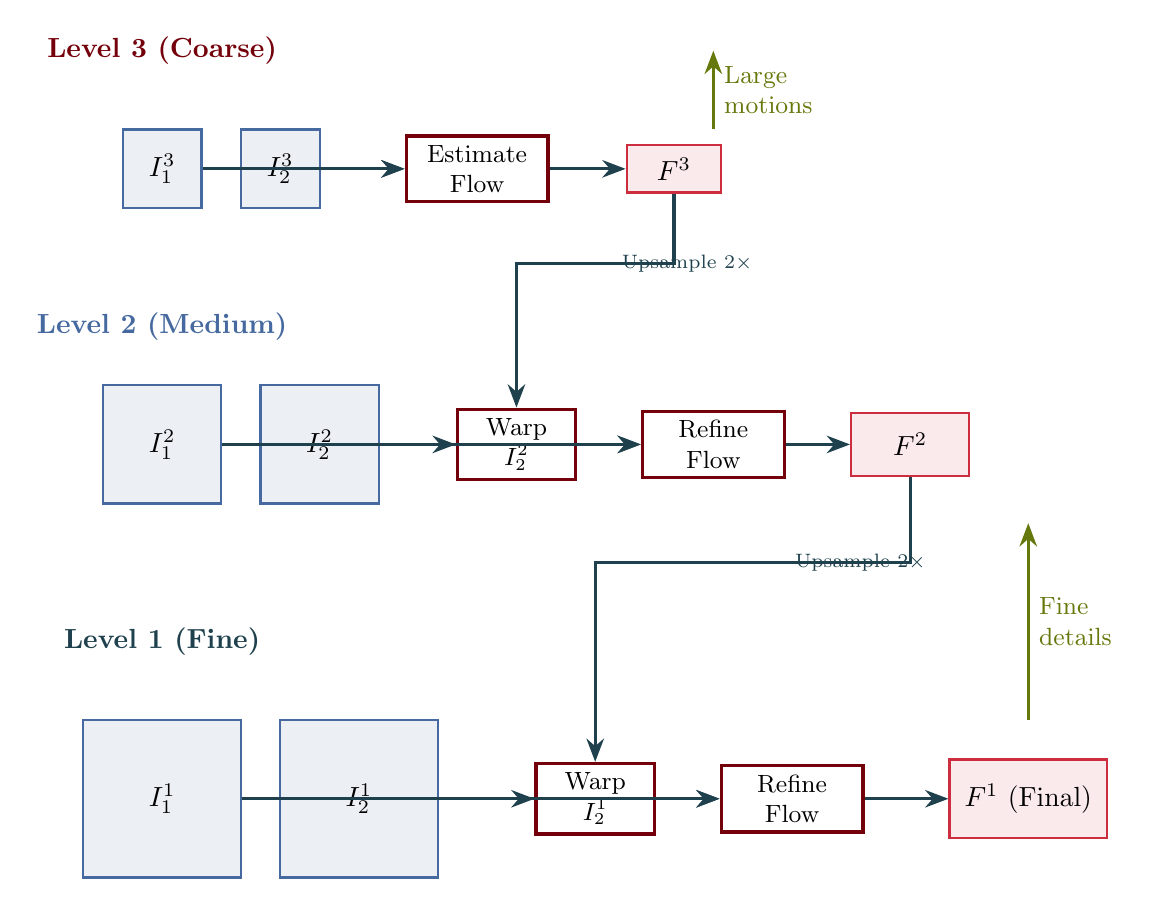
\begin{tikzpicture}[>=Stealth,
    box/.style={rectangle, draw=garnet, very thick, fill=white, minimum width=1.8cm, minimum height=0.8cm, align=center, font=\small},
    img/.style={rectangle, draw=atlantic, thick, fill=atlantic!10},
    arrow/.style={->, very thick, congaree}]

    % Level 3 (Coarse)
    \node[font=\bfseries, garnet] at (0,5) {Level 3 (Coarse)};
    \node[img, minimum width=1cm, minimum height=1cm] (img3a) at (0,3.5) {$I_1^3$};
    \node[img, minimum width=1cm, minimum height=1cm] (img3b) at (1.5,3.5) {$I_2^3$};
    \node[box] (est3) at (4,3.5) {Estimate\\Flow};
    \node[img, minimum width=1.2cm, minimum height=0.6cm, fill=rose!10, draw=rose] (flow3) at (6.5,3.5) {$F^3$};

    \draw[arrow] (img3a) -- (est3);
    \draw[arrow] (img3b) -- (est3);
    \draw[arrow] (est3) -- (flow3);

    % Level 2 (Medium)
    \node[font=\bfseries, atlantic] at (0,1.5) {Level 2 (Medium)};
    \node[img, minimum width=1.5cm, minimum height=1.5cm] (img2a) at (0,0) {$I_1^2$};
    \node[img, minimum width=1.5cm, minimum height=1.5cm] (img2b) at (2,0) {$I_2^2$};
    \node[box, minimum width=1.5cm] (warp2) at (4.5,0) {Warp\\$I_2^2$};
    \node[box] (est2) at (7,0) {Refine\\Flow};
    \node[img, minimum width=1.5cm, minimum height=0.8cm, fill=rose!10, draw=rose] (flow2) at (9.5,0) {$F^2$};

    \draw[arrow] (flow3) -- ++(0,-1.2) -| node[pos=0.2, right, font=\scriptsize] {Upsample $2\times$} (warp2);
    \draw[arrow] (img2a) -- (est2);
    \draw[arrow] (img2b) -- (warp2);
    \draw[arrow] (warp2) -- (est2);
    \draw[arrow] (est2) -- (flow2);

    % Level 1 (Fine)
    \node[font=\bfseries, congaree] at (0,-2.5) {Level 1 (Fine)};
    \node[img, minimum width=2cm, minimum height=2cm] (img1a) at (0,-4.5) {$I_1^1$};
    \node[img, minimum width=2cm, minimum height=2cm] (img1b) at (2.5,-4.5) {$I_2^1$};
    \node[box, minimum width=1.5cm] (warp1) at (5.5,-4.5) {Warp\\$I_2^1$};
    \node[box] (est1) at (8,-4.5) {Refine\\Flow};
    \node[img, minimum width=2cm, minimum height=1cm, fill=rose!10, draw=rose] (flow1) at (11,-4.5) {$F^1$ (Final)};

    \draw[arrow] (flow2) -- ++(0,-1.5) -| node[pos=0.2, right, font=\scriptsize] {Upsample $2\times$} (warp1);
    \draw[arrow] (img1a) -- (est1);
    \draw[arrow] (img1b) -- (warp1);
    \draw[arrow] (warp1) -- (est1);
    \draw[arrow] (est1) -- (flow1);

    % Side annotation
    \draw[<-, very thick, horseshoe] (7,5) -- (7,4) node[midway, right, align=left, font=\small] {Large\\motions};
    \draw[<-, very thick, horseshoe] (11,-1) -- (11,-3.5) node[midway, right, align=left, font=\small] {Fine\\details};

\end{tikzpicture}
\end{document}
